\documentclass[tikz, border=5mm]{standalone}
\usepackage{tikz}
\usepackage{amsmath}
\begin{document}

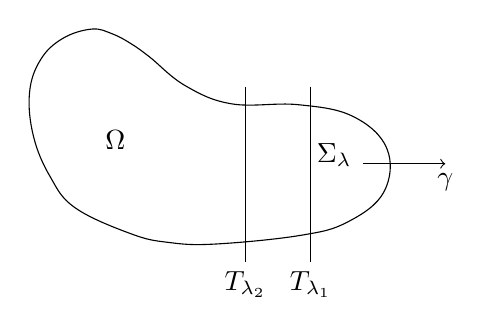
\begin{tikzpicture}
\draw plot [smooth cycle, tension=0.65] coordinates {(-2.49,1.84) (-2.12, 1.96) (-1.86, 1.9) (-1.63, 1.78) (-1.39, 1.61) (-0.93, 1.24) (-0.34, 1.01) (0.5, 1) (1.2, 0.85) (1.63, 0.44) (1.59, -0.11) (1.13, -0.49) (0.53, -0.66) (-0.55, -0.77) (-1.14, -0.75) (-1.62, -0.64) (-2.33, -0.31) (-2.65, 0.09) (-2.86, 0.6) (-2.91, 1.15) (-2.77, 1.57)};
\draw (-0.17, 1.22)--(-0.17, -1) node[below] {$T_{\lambda_2}$};
\draw (0.66, 1.23)--(0.66, -1) node[below] {$T_{\lambda_1}$};
\node at (0.96, 0.36) {$\Sigma_{\lambda}$};
\draw [->] (1.33, 0.25)--(2.37, 0.25) node[below] {$\gamma$};
\node at (-1.82, 0.55) {$\Omega$};
\end{tikzpicture}
\end{document}